%Version 3.1 December 2024
% StretchBot: Neuro-Symbolic Planning for Adaptive Assistive Robot Guidance
% Springer Nature Journal Submission
%
%%%%%%%%%%%%%%%%%%%%%%%%%%%%%%%%%%%%%%%%%%%%%%%%%%%%%%%%%%%%%%%%%%%

\documentclass[pdflatex,sn-basic,Numbered,iicol,twocolumn]{sn-jnl}% KI/Springer layout with numbered citations and two-column formatting

\usepackage{graphicx}%
\usepackage{amsmath,amssymb,amsfonts}%
\usepackage{amsthm}%
\usepackage{mathrsfs}%
\usepackage[title]{appendix}%
\usepackage{xcolor}%
\usepackage{textcomp}%
\usepackage{booktabs}%

\raggedbottom

\begin{document}

\title[StretchBot: Neuro-Symbolic Planning for Adaptive Assistive Robot Guidance]{StretchBot: Neuro-Symbolic Planning for Adaptive Assistive Robot Guidance}

\author*[1]{\fnm{Luca} \sur{Vogelgesang}}\email{luca.vogelgesang@etu.umontpellier.fr}

\author*[1]{\fnm{Mehdi} \sur{Alvi}}\email{soltaniahmedmehdi@gmail.com}

\author[1]{\fnm{Xinrui} \sur{Zu}}\email{x.zu@vu.nl}

\author[1]{\fnm{Stefano} \sur{De Giorgis}}\email{stefano.de.giorgis@gmail.com}

\author[1]{\fnm{Mohammadhossein} \sur{Khojasteh}}\email{mohammadhosseinkhojaste@gmail.com}

\author[1]{\fnm{Filip} \sur{Ilievski}}\email{f.ilievski@vu.nl}

\affil*[1]{\orgdiv{Faculty of Science, Department of Computer Science}, \orgname{Vrije Universiteit Amsterdam}, \orgaddress{\street{De Boelelaan 1081a}, \city{Amsterdam}, \postcode{1081 HV}, \country{Netherlands}}}

\abstract{
Assistive robots used in home and health settings need to adapt to user state and environmental context while preserving safe and coherent behavior. We present StretchBot, a neuro-symbolic coaching system for guided stretching routines. The method combines structured knowledge representation with large language models and multimodal perception, including object detection, facial and vocal affect cues, posture monitoring, and speech transcription. Perception outputs are fused into a contextual state that is enriched with knowledge graph relations and then used for adaptive action selection. A verification stage checks response format and interaction tone before execution, and the handler maps validated outputs to robot actions such as progressing to the next exercise or pointing to a relevant object. We report a pilot proof-of-concept evaluation with three participants comparing scripted and adaptive conditions. Descriptive results indicate higher perceived adaptability and object relevance in the adaptive condition, while scripted interaction remains competitive for smoothness and predictability. These findings support the practical value of actionable knowledge representation for grounding learned reasoning into embodied robot behavior, and they motivate larger studies to evaluate generalizability and long-term user outcomes.
}

\keywords{Neuro-Symbolic AI, Large Language Models, Knowledge Graphs, Assistive Robotics, Adaptive Planning, Human-Robot Interaction}

\maketitle

\section{Introduction}
\label{sec:intro}

Robotic systems are increasingly deployed in domestic and healthcare environments to support human wellbeing through physical assistance, rehabilitation, and guided exercise routines \cite{ref1,ref2}. Among these, assistive stretching robots have shown potential for improving flexibility, reducing stress, and encouraging physical activity in daily life \cite{ref3}. However, most existing systems remain scripted and inflexible, providing limited personalization to the user's physical state, emotional condition, or surrounding context \cite{ref4}. This lack of adaptation can reduce engagement, hinder safety, and limit long-term adoption.

The fundamental challenge lies in balancing two competing demands: (1) \textit{structured predictability}—a clear script that ensures comprehensive exercise coverage and user confidence, and (2) \textit{contextual responsiveness}—real-time adaptation to the user's current state, emotions, and environment. Purely scripted systems excel at predictability but fail to personalize. Fully reactive systems can adapt but risk incoherence and repeated exercises.

To address these challenges, this work investigates whether and how adaptive robotic guidance can outperform scripted routines in terms of personalization, naturalness, and contextual relevance. We examine to what extent multimodal perception combined with commonsense reasoning enables a robot to adapt its guidance to the user's state and environment. Building on this research question, we developed \textbf{StretchBot}, an adaptive robotic coach designed to guide users through a short morning stretching routine while dynamically adjusting its behavior to real-time multimodal cues.

StretchBot integrates perception, commonsense reasoning, and interaction control in a unified architecture, enabling it to perceive user state through voice, facial expression, and posture, detect relevant objects in the environment, and adapt stretching plans accordingly. At its core lies a \textit{hybrid reasoning module} that couples a knowledge graph encoding causal, temporal, and affordance-based relations with a large language model (LLM) for context-aware decision-making \cite{ref5,ref26}. This reasoning pipeline is augmented with a verification loop using a secondary language model to ensure safety, protocol adherence, and empathetic communication before actions are executed \cite{ref28}.

\subsection{Terminology and Abbreviations}

Because this paper targets a general artificial intelligence readership, we briefly clarify key terms used throughout the manuscript. A \textit{knowledge graph} is a structured network of entities and relations (for example, \texttt{coffee -> reduces -> fatigue}) that supports explicit reasoning. \textit{ConceptNet} is a public commonsense knowledge base that stores broad everyday relations and is used here as a fallback when domain-specific knowledge is missing. \textit{Neuro-symbolic} refers to combining learned models (neural components) with explicit symbolic structures (rule-like or graph-based knowledge). \textit{Embodied action} means that system decisions are not only textual outputs but are executed physically by a robot in the environment.

We use the following abbreviations consistently: \textit{LLM} (large language model), \textit{KG} (knowledge graph), \textit{STT} (speech-to-text), and \textit{TTS} (text-to-speech).

\subsection{Research Questions and Contributions}

Our work addresses three core research questions:

\textbf{RQ1:} Can a hybrid neuro-symbolic architecture (LLM + knowledge graph) enable effective plan adaptation in assistive robotics?

\textbf{RQ2:} How should actionable knowledge be represented and integrated with LLM reasoning to ground robot decisions in both perception and domain knowledge?

\textbf{RQ3:} Do users perceive adaptive robot guidance as preferable to scripted routines, and in which dimensions?

The main contributions of this work are:

\begin{enumerate}
\item An adaptive stretching robot framework integrating multimodal perception (emotion recognition, object detection, posture estimation), commonsense reasoning, and interaction control for guided physical routines.

\item Integration of knowledge graph reasoning with large language model prompt design, enabling the robot to adapt exercise plans based on user state, environment, and prior interaction history.

\item A collaborative interaction protocol ensuring explicit user confirmation before all actions, balancing proactive adaptation with human oversight.

\item Comparative human evaluation of scripted versus adaptive guidance in a real-world stretching scenario, with quantitative ratings and qualitative feedback.

\item Analysis of strengths and limitations of hybrid LLM-KG planning for assistive robotics, with implications for future neuro-symbolic systems.
\end{enumerate}
\section{Related Work}
\label{sec:related}

Our work sits at the intersection of four research areas: assistive robotics, commonsense reasoning, multimodal interaction, and LLM-based planning.

\subsection{Assistive Robotics for Physical Guidance}

Robots have been explored as assistants for stretching and rehabilitation exercises, aiming to improve user wellbeing and engagement. Previous work \cite{ref6} showed that scripted stretching robots can help users maintain focus and reduce stress during routines. However, such systems are limited by their lack of real-time adaptation to user state. Another study \cite{ref7} proposed a rehabilitation robot for Parkinson's patients that adapted exercises over time, but the adaptation relied on fixed predefined rules. In contrast, StretchBot combines multimodal perception with commonsense reasoning to adapt instructions continuously during a session, allowing for more personalized and context-aware guidance.

Key challenges in assistive robotics include ensuring safety while granting autonomy, personalizing guidance to individual needs, and maintaining user engagement over time. Our approach addresses these by coupling structured exercise baselines with adaptive branching points.

\subsection{Commonsense Reasoning and Knowledge Graphs}

Commonsense reasoning has been used to give robots a better understanding of their environment and the needs of the user \cite{ref8}. Prior work \cite{ref8} proposed multiple dimensions of commonsense knowledge, which inspired the organization of our knowledge graph. Another study \cite{ref9} showed that combining symbolic planning with language models can fill gaps in action reasoning. In our case, commonsense reasoning is applied to connect perceived user states—such as fatigue or thirst—with relevant object affordances, allowing the robot to decide when to suggest a break or indicate a helpful object.

Knowledge graphs provide interpretability and structured reasoning compared to unstructured language models alone. By coupling KGs with LLMs, we leverage both the explainability of symbolic systems and the flexibility of neural language models.

\subsection{Multimodal Interaction in Human-Robot Interaction}

Prior work has shown that combining multiple sensing modalities improves the adaptability and perceived quality of human-robot interaction \cite{ref10}. For example, researchers \cite{ref10} used emotion and posture detection to adjust guidance, while other work \cite{ref11} adapted robot behavior in response to signs of fatigue. StretchBot integrates emotion, posture, and environmental object cues into a reasoning process that supports timely and context-aware assistance, such as proposing a pause or pointing to a relevant object.

The fusion of multiple modalities also increases robustness: transient errors in one modality can be compensated by others, improving overall reliability.

\subsection{LLM-Based Planning and Reasoning}

Recent work has explored the use of large language models for robotic planning \cite{ref12}. One approach \cite{ref12} introduced SayCan, combining LLM-based reasoning with affordance detection to generate feasible action plans. Another study \cite{ref13} demonstrated that maintaining an ``inner monologue'' allows LLMs to revise plans in real time, increasing success rates. Several surveys \cite{ref14} have identified strengths and weaknesses of LLM reasoning, while recent contributions have highlighted the need for hybrid approaches \cite{ref15}. StretchBot applies these insights to the domain of physical guidance, coupling LLMs with a structured knowledge graph and a verification loop to ensure safe, empathetic, and contextually appropriate robot actions.
\section{System Architecture}
\label{sec:architecture}

StretchBot is structured around a four-stage pipeline: Perception, Reasoning, Action Execution, and Planning \& Adaptation. Each stage transforms information into increasingly higher-level representations, enabling the robot to adapt its behavior in real time. Figure~\ref{fig:overall_pipeline} summarizes this closed control loop and the direction of information flow.

\begin{figure*}[t]
\centering
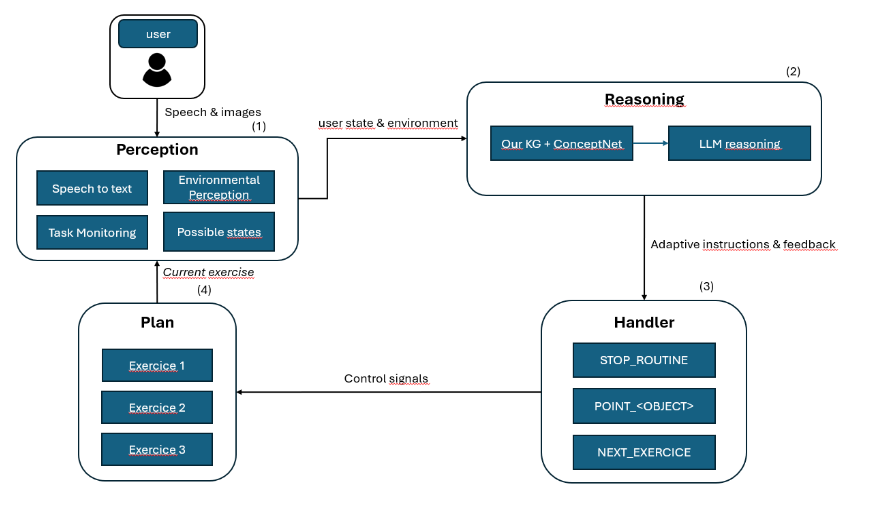
\includegraphics[width=0.92\textwidth]{../images/figure1_pipeline.png}
\caption{Overall StretchBot pipeline organized into four stages: Perception, Reasoning, Action Execution (Handler), and Planning \& Adaptation. The numbered markers indicate the main flow steps discussed in the text.}
\label{fig:overall_pipeline}
\end{figure*}

The numbered markers in Figure~\ref{fig:overall_pipeline} correspond to the operational sequence used in our implementation. Marker \textbf{(1)} denotes the multimodal input transfer from the user to the \textit{Perception} block (speech and image streams). Marker \textbf{(2)} denotes the transition from perceived user/environment state to the \textit{Reasoning} block, where KG + ConceptNet context is combined with LLM reasoning. Marker \textbf{(3)} denotes the delivery of adaptive instructions and feedback from \textit{Reasoning} to the \textit{Handler} (execution interface using actions such as \texttt{NEXT\_EXERCISE}, \texttt{POINT\_<OBJECT>}, and \texttt{STOP\_ROUTINE}). Marker \textbf{(4)} denotes the control feedback from the Handler to the \textit{Plan} block, which updates the current exercise stage and closes the adaptation loop.

\subsection{Perception Module}

In Figure~\ref{fig:overall_pipeline}, this module is the left block and corresponds to the first stage of the loop. The perception module provides the adaptive system with a continuous and multimodal understanding of both the user's state and the environment. It integrates four complementary components:

\subsubsection{Object Detection}
Visual scene analysis is performed using YOLOv8 \cite{ref18}, applied to the live RGB feed from the robot's camera. The system retrieves the complete list of all detected objects in the scene and sends this list to the reasoning module, ensuring that every recognized element is available for potential reasoning or adaptation.

\subsubsection{Multimodal Emotion Recognition}
The user's emotional state is inferred through the fusion of three independent detection channels:
\begin{itemize}
\item \textit{Voice emotion recognition}—using a HuggingFace Transformers pipeline \cite{ref19} on speech segments captured by the microphone.
\item \textit{Facial emotion recognition}—using DeepFace \cite{ref20} applied to the video stream.
\item \textit{Text-based emotion recognition}—using a lightweight HuggingFace model \cite{ref19} on transcribed speech.
\end{itemize}

A dedicated fusion module performs weighted fusion and majority voting to produce a single aggregated emotional state, which is then summarized in natural language for the LLM.

\subsubsection{Task Monitoring}
Task monitoring verifies, in real time, that the user is correctly performing each stretching exercise and holding the required pose for the prescribed duration. It relies on \textbf{MediaPipe Pose} \cite{ref21}, a lightweight skeleton-estimation library that infers the positions of 33 body landmarks (shoulders, elbows, wrists, hips, ankles, etc.) from a single RGB frame at 30\,Hz.

\paragraph{Per-exercise pose criteria.}
Each exercise is evaluated by a dedicated geometric check applied to the MediaPipe landmark coordinates:

\begin{itemize}
\item \textit{Arms above the head.} The system checks that both wrists and both elbows have a $y$-coordinate strictly lower than the nose landmark ($y_\text{wrist} < y_\text{nose}$ and $y_\text{elbow} < y_\text{nose}$, where lower $y$ means higher in the frame), and that the horizontal distance between the two wrists is below a threshold $w_\text{max} = 0.3$ (in normalised image coordinates), ensuring the arms are raised and approximately centred above the head.

\item \textit{Touch-your-toes.} The system computes the Euclidean distance in normalised image coordinates between each wrist landmark and each ankle landmark:
\begin{equation}
d_{ij} = \sqrt{(x_{\text{wrist},i} - x_{\text{ankle},j})^2 + (y_{\text{wrist},i} - y_{\text{ankle},j})^2}\,,
\label{eq:toe_distance}
\end{equation}
and accepts the pose when any $d_{ij} < 0.4$.

\item \textit{Lateral trunk lean (left / right).} The system computes the midpoint of the shoulders $M_s$ and the midpoint of the hips $M_h$, then calculates the signed trunk inclination angle:
\begin{equation}
\alpha = \arctan\!\left(\frac{M_{s,x} - M_{h,x}}{M_{h,y} - M_{s,y}}\right),
\label{eq:trunk_angle}
\end{equation}
where the $y$-axis inversion accounts for OpenCV's top-down coordinate origin. The user is classified as leaning \textit{right} when $\alpha > 15^\circ$ and \textit{left} when $\alpha < -15^\circ$.
\end{itemize}

\paragraph{Hold-duration accumulation and reset.}
At each valid frame the hold timer is incremented by the fixed frame period $\Delta t = 1/30\,\text{s}$, capped at the target duration $T = 5\,\text{s}$. If the user holds an invalid pose for longer than a reset tolerance of $t_\text{reset} = 40\,\text{s}$, the timer is zeroed and corrective spoken feedback is issued via the TTS channel. Once the timer reaches $T$, the task monitor emits a success event that propagates via markers \textbf{(3)} and \textbf{(4)} in Figure~\ref{fig:overall_pipeline}.

For the lateral lean exercise, two independent timers track the left-side and right-side hold durations; both must reach $T = 5\,\text{s}$ before the exercise is marked complete.

All pose checks are purely geometric and frame-local, requiring no additional training data beyond the pre-trained MediaPipe model.

\subsubsection{Speech-to-Text (STT)}
The STT component converts the user's spoken input into text for downstream processing. Vosk \cite{ref22} was initially used due to its lightweight local deployment, with Google Cloud Speech-to-Text \cite{ref23} considered for higher accuracy.

All perception outputs are structured into a unified context package containing the detected objects, the aggregated emotional state, the current task execution status, and the most recent STT transcript. This package operationalizes marker \textbf{(1)} and is transmitted to the reasoning block through marker \textbf{(2)} in Figure~\ref{fig:overall_pipeline}.

\subsection{Reasoning Module}

In Figure~\ref{fig:overall_pipeline}, this module is the upper-right block that receives the perception context through marker \textbf{(2)} and sends actionable output to the handler through marker \textbf{(3)}. The reasoning module serves as the central decision-making component, responsible for determining the robot's next action by combining perception outputs, prior knowledge, and the predefined stretching routine. Its operation follows a hybrid approach: rule-based checks handle explicitly defined conditions, while an LLM provides high-level reasoning, contextual adaptation, and natural-language interaction.

\subsubsection{Context Integration and Knowledge Graph Retrieval}

Each time the user speaks, the reasoning module compiles an updated context package including:
\begin{itemize}
\item the list of objects detected by perception,
\item the aggregated emotional state,
\item the current exercise progress status,
\item the latest speech-to-text transcription.
\end{itemize}

To provide the LLM with meaningful background knowledge, this raw context is enriched with semantic relations retrieved from a Knowledge Graph (KG). A knowledge graph is a structured representation of concepts (nodes) and their relationships (edges), often expressed as triples like (coffee, reduces, fatigue) \cite{ref26}. Unlike unstructured text, a KG enables the system to reason over entities and their connections in a transparent and interpretable way.

\subsubsection{LLM-Based Adaptive Reasoning}

The complete context package is passed to the primary LLM through a structured prompt. The model analyzes this information to decide the most appropriate next step in the stretching session, adapting the style and tone of its response to match the detected emotional state. If relevant objects are available in the scene, the model may refer to them directly in its suggestions.

The LLM adheres to predefined action prefixes in its outputs:
\begin{itemize}
\item \texttt{NEXT\_EXERCISE:} instructs the system to move to the following stretch.
\item \texttt{POINT\_<OBJECT>:} directs the robot to point to a detected object.
\item \texttt{STOP\_ROUTINE:} ends the stretching session.
\end{itemize}

\subsubsection{Response Verification}

Once the primary LLM has generated a response, it is passed to a secondary, smaller LLM acting as a verifier. This verification stage maintains the quality and consistency of interactions by checking the message format, confirming appropriate tone, and ensuring coherence with the current session context. The verified output is then emitted as adaptive instructions and feedback, which corresponds directly to marker \textbf{(3)} in Figure~\ref{fig:overall_pipeline}.

\subsection{Action Execution Module}

This module corresponds to the \textit{Handler} block in Figure~\ref{fig:overall_pipeline}. The action execution module grounds high-level reasoning decisions in concrete robot behavior. It acts as the interface between symbolic instructions and the physical world, ensuring that every action is carried out in a synchronized, safe, and comprehensible manner.

\subsubsection{Command Interpretation}
Each output from the reasoning stage arrives in dual format: a structured action prefix and a natural-language sentence. The action prefix encodes the intended behavior in machine-readable form, while the text provides a human-friendly explanation.

\subsubsection{Physical Execution of Movements}
Once a symbolic command such as \texttt{POINT\_Coffee} has been issued, the system translates it into a fixed Cartesian target pose. The target is passed to MoveIt \cite{ref31}, which computes a feasible joint-space trajectory while avoiding collisions. The trajectory is optimized using cubic spline interpolation \cite{ref32} to ensure smooth and continuous motion.

The final optimized trajectory is executed step by step on the Lynxmotion SES900 arm \cite{ref33}. Once the target pose is reached within tolerance, an ``execution finished'' event is published back to the reasoning module.

\subsubsection{Verbal Feedback and Synchronization}
In parallel with motion control, text-to-speech (TTS) converts the LLM's natural-language output into spoken instructions. The timing of speech and movement is carefully coordinated to enhance clarity and naturalness of the interaction \cite{ref34}. The system supports multiple voices, ranging from simple rule-based synthesis to expressive neural voices capable of conveying emotion \cite{ref35}, reinforcing empathy and engagement.

\subsubsection{Safety Supervision}
A critical aspect of execution is maintaining user safety and hardware integrity. The module integrates a watchdog subsystem that supervises all ongoing actions:
\begin{itemize}
\item Joint limits and velocity clamping prevent excessive extension or unsafe speed.
\item Collision detection monitors the environment for potential collisions.
\item Emergency stop immediately halts execution if anomalies are detected.
\end{itemize}

After execution status is updated, the handler sends control feedback to the planning block, implementing marker \textbf{(4)} in Figure~\ref{fig:overall_pipeline}.

\subsection{Planning and Adaptation Module}

In Figure~\ref{fig:overall_pipeline}, this module is the lower-left \textit{Plan} block. It receives control feedback from the handler via marker \textbf{(4)} and maintains the current exercise state that is fed back into perception for the next cycle. The planning and adaptation module ensures that StretchBot delivers a stretching session that is both structured and responsive.

\subsubsection{Global Routine Structure}
At its core, the system relies on a predefined exercise script composed of a sequence of stretching primitives (e.g., arm stretch, side bend, neck rotation). Each primitive specifies the expected body posture, target hold duration (5 s), and the transition to the next exercise. This script acts as a baseline plan that guarantees coverage and maintains a clear flow.

\subsubsection{Local Adaptations}
On top of this baseline, the system introduces adaptive branching points where the flow can be adjusted depending on the user's state. For example:

\begin{itemize}
\item If the user reports fatigue, the system may suggest a brief pause or recommend a coffee break while maintaining the overall sequence.
\item If the user expresses discomfort with a particular stretch, the system can substitute a gentler alternative or skip to the next exercise.
\item If relevant objects are detected in the environment, the system proactively offers suggestions (e.g., ``I see a bottle of water nearby—would you like a sip?'').
\end{itemize}

These adaptations occur within the framework of the global routine, ensuring that the session remains coherent and goal-directed while accommodating individual preferences and states. Together, markers \textbf{(1)} to \textbf{(4)} therefore describe one complete adaptation cycle that readers can follow in parallel with this section.
\section{Implementation}
\label{sec:implementation}

\subsection{Software Stack}

StretchBot is built on a modular software architecture using Robot Operating System 2 (ROS2) to coordinate communication between perception, reasoning, and execution components. Key libraries include:

\begin{itemize}
\item \textbf{Perception:} YOLOv8n (``You Only Look Once'', version 8, nano variant) for real-time object detection; \textbf{MediaPipe Pose} for skeleton landmark extraction and pose verification; DeepFace for facial emotion recognition; HuggingFace Transformers pipelines for voice-segment and transcript-level emotion analysis.
\item \textbf{Reasoning:} Custom Python modules for KG retrieval and context integration; open-weight large language models served through the \textbf{OpenRouter API} (specifically DeepSeek-R1 as primary reasoning model and Llama-3.3-Nemotron-49B as the configured production model) for LLM-based planning; a secondary LLM accessed via the \textbf{HuggingFace Inference Client} (nscale provider) for output verification.
\item \textbf{Execution:} MoveIt~2 for trajectory planning; \textbf{Vosk} with the \texttt{vosk-model-small-en-us-0.15} acoustic model for local, offline speech-to-text; \textbf{gTTS} (Google Text-to-Speech Python library) for standard speech synthesis and a HuggingFace Gradio TTS space for expressive, emotion-aware neural voices.
\item \textbf{Spatial Perception:} \textbf{ArUco markers} (4×4 50-dictionary, OpenCV) combined with camera calibration for metric 3-D pose estimation of objects, enabling precise pointing commands.
\item \textbf{Hardware Communication:} ROS2 (\texttt{rclpy}) with a dedicated node (\texttt{llm\_commander}) publishing symbolic commands on the \texttt{target\_point} topic; low-level drivers for the Lynxmotion SES900 arm.
\end{itemize}

A key architectural decision is the \textbf{concurrent execution} of LLM reasoning and pose monitoring. The LLM interaction runs in a dedicated Python thread, continuously accepting speech input and generating adaptive responses, while the main thread executes the real-time MediaPipe pose-tracking loop at 30\,Hz. An \texttt{exercise\_done} flag and a \texttt{stop\_flag} dictionary coordinate termination between the two threads.

\subsection{Prompt Engineering and Response Format}

The primary LLM is instructed through a comprehensive system prompt that provides context about the user, the stretching routine, detected objects, and emotional state. The prompt explicitly instructs the model to use predefined action prefixes and to adapt its tone based on the user's emotional state. The format ensures consistent machine-readable output while maintaining natural language quality.

Example system prompt fragment:
\begin{quote}
\small\ttfamily
You are a friendly and empathetic stretching assistant.\\
The user is currently [emotional\_state].\\
Detected objects in the room are: [objects].\\
The current exercise is [exercise\_name], and the user status is [status].\\
Use one of these action prefixes when relevant:\\
NEXT\_EXERCISE, POINT\_<OBJECT>, STOP\_ROUTINE.\\
Always be encouraging and personalized.\\
Respond naturally, adapting your tone to the user's emotion.
\end{quote}

\subsection{Knowledge Representation}

The internal knowledge graph is implemented as a structured \textbf{JSON file} (\texttt{knowledge\_graph.json}) parsed at runtime into Python dictionaries. Each entity entry stores a \texttt{relations} dictionary mapping predicate names to values or lists of values — a lightweight alternative to a full RDF triple store that keeps the system dependency-free. Key relations include:

\begin{itemize}
\item \textit{Entity-Property relations:} \texttt{(coffee, hasAffect, energizes)}, \texttt{(water, hasAffect, hydrates)}.
\item \textit{Emotion-Response relations:} \texttt{(tired, suggests, break)}, \texttt{(tired, suggests, caffeine)}.
\item \textit{Exercise-Benefit relations:} \texttt{(arm\_stretch, improves, shoulder\_flexibility)}.
\item \textit{Affordance relations:} \texttt{(coffee, usedFor, energy\_boost)}, \texttt{(wall, usedFor, balance\_support)}.
\end{itemize}

When an entity or state is not found in the internal KG, the system queries the ConceptNet API to retrieve commonsense relations, filtering by the relation types \texttt{UsedFor}, \texttt{Causes}, \texttt{HasProperty}, \texttt{MotivatedByGoal}, and \texttt{IsA}.

\subsection{Hardware Setup}

The system is integrated with a Lynxmotion SES900 robotic arm mounted on a wheeled mobile base (optional). The robot is equipped with:
\begin{itemize}
\item An Intel RealSense RGB-D camera for object detection and posture estimation.
\item A microphone array for speech capture and emotion recognition.
\item Speakers for speech synthesis.
\item Torque sensors on the arm for safety monitoring.
\end{itemize}
\section{Proof-of-Concept and Pilot Evaluation}
\label{sec:evaluation}

\subsection{Evaluation Design}

We conducted a proof-of-concept comparative user study contrasting a scripted baseline with the adaptive system. The study design was a within-subjects pilot comparison where participants experienced both conditions in counterbalanced order.

\subsection{Participants and Protocol}

Three participants (P1, P2, P3) aged 28–35 participated in the pilot study. Each participant completed two stretching sessions, each lasting approximately 8–10 minutes: (1) a scripted baseline condition where the robot followed a fixed exercise sequence without perception-based adaptation, and (2) the adaptive condition where the robot adjusted guidance based on user state and environment.

A two-minute break separated the two conditions. Participants were informed of the study's purpose and signed informed consent forms. The study was conducted in a controlled laboratory environment with standard objects present (coffee mug, water bottle, banana, chair).

\subsection{Quantitative Metrics}

After each condition, participants completed a custom questionnaire rating the robot's performance on six dimensions:

\begin{enumerate}
\item \textbf{Clarity:} How clear were the robot's instructions? (1–5 Likert scale)
\item \textbf{Comfort:} How comfortable were you during the routine? (1–5)
\item \textbf{Adaptability:} How well did the robot adapt to your state and needs? (1–5)
\item \textbf{Trust:} How much did you trust the robot's decisions? (1–5)
\item \textbf{Naturalness:} How natural and human-like was the robot's behavior? (1–5)
\item \textbf{Object Relevance:} How relevant were the robot's object suggestions? (1–5, N/A for scripted condition)
\end{enumerate}

Additionally, we recorded:
\begin{itemize}
\item Task completion time (total session duration).
\item Number of user interventions (corrections or clarifications requested).
\item Number of LLM reasoning cycles per session.
\item Latency of adaptive responses (time from user input to robot output).
\end{itemize}

\subsection{Qualitative Feedback}

After completing both conditions, participants participated in semi-structured interviews (15–20 minutes) discussing:
\begin{itemize}
\item Which version they preferred and why.
\item Perceived strengths and weaknesses of each approach.
\item Suggestions for improvement.
\item Overall sense of engagement and repeated-use intentions.
\end{itemize}

All interviews were recorded, transcribed, and analyzed using thematic coding by two independent raters. Inter-rater agreement (Cohen's kappa) was monitored to ensure consistency.

\subsection{Planned Analysis for a Full-Scale Study}

To move beyond pilot-level evidence, the next evaluation phase will use a pre-registered analysis plan. The primary endpoint will be perceived adaptability, with secondary endpoints including trust, naturalness, completion time, and intervention count. For subjective outcomes, we will use mixed-effects models with participant-level random intercepts to account for repeated measures. For non-normal outcomes (e.g., count-based interventions), we will use generalized mixed-effects models.

We will also report effect sizes and confidence intervals in addition to p-values, and include multiple-comparison correction for secondary outcomes. This design will allow us to test whether the trends observed in this pilot remain stable at larger scale while preserving ecological validity.
\section{Results}
\label{sec:results}

\subsection{Quantitative Results}

Given the small pilot sample ($N=3$), we report descriptive statistics and preliminary trends rather than inferential statistical claims.

\textbf{Clarity:} Both conditions were rated highly for clarity (Scripted: $M=4.67, SD=0.33$; Adaptive: $M=4.33, SD=0.67$). The scripted version had a slight advantage, likely due to its predictability.

\textbf{Comfort:} Ratings were comparable across conditions (Scripted: $M=4.33, SD=0.67$; Adaptive: $M=4.00, SD=0.82$). Both systems were perceived as comfortable environments for stretching.

\textbf{Adaptability:} In our small sample, the adaptive system received higher ratings ($M=4.33, SD=0.67$) than the scripted system ($M=2.00, SD=0.82$), indicating a strong preliminary trend in favor of context-sensitive guidance.

\textbf{Trust:} Trust ratings were similar between conditions (Scripted: $M=4.33, SD=0.67$; Adaptive: $M=4.00, SD=0.82$), suggesting that the verification loop and safety measures effectively maintained user confidence.

\textbf{Naturalness:} The adaptive system was rated slightly higher for naturalness (Adaptive: $M=4.33, SD=0.33$; Scripted: $M=3.67, SD=0.89$), indicating better human-like interaction.

\textbf{Object Relevance:} In the adaptive condition, object suggestions were rated as highly relevant ($M=4.67, SD=0.33$), demonstrating the effectiveness of the KG-LLM integration.

\begin{figure*}[t]
\centering
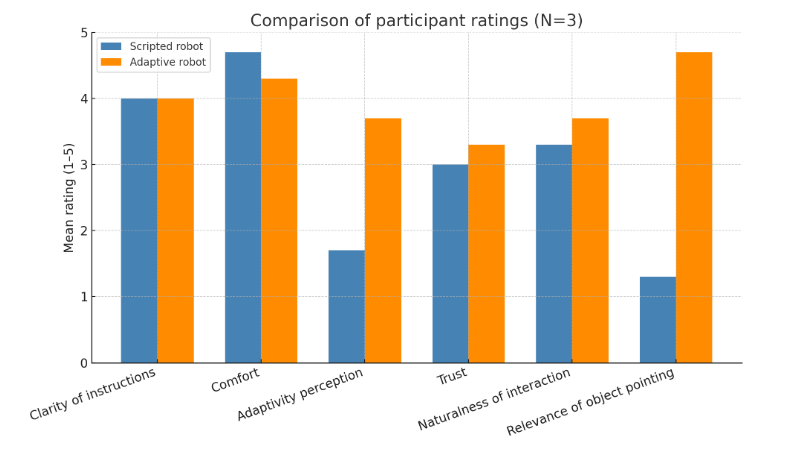
\includegraphics[width=0.88\textwidth]{../images/figure3_results.png}
\caption{Comparative results between scripted and adaptive conditions across the main user-evaluation dimensions.}
\label{fig:comparative_results}
\end{figure*}

Figure~\ref{fig:comparative_results} visualizes the rating profile of both conditions and highlights the same trend observed in the numerical analysis: the adaptive system clearly outperforms the scripted baseline on \textit{adaptivity perception} and \textit{relevance of object pointing}, while \textit{clarity} and \textit{comfort} remain similar or slightly in favor of the scripted mode. This pattern supports our main claim that adaptation improves contextual relevance, but does not automatically guarantee a smoother interaction experience.

\subsection{Response Latency}

Average task completion time was similar between conditions (Scripted: $M=487s, SD=31s$; Adaptive: $M=512s, SD=58s$), with the adaptive system taking slightly longer due to LLM reasoning overhead. In this pilot setting, the observed latency remained within acceptable ranges (mean latency per response: $\approx2$–$3$ seconds).

\subsection{Qualitative Findings}

\textbf{Preference:} Two participants (P2, P3) preferred the scripted version, citing predictability, smoother flow, and lower cognitive load. One participant (P1) preferred the adaptive version, appreciating its personalization and environmental awareness.

\textbf{Strengths of Adaptive System:} Participants noted that the adaptive system was ``more thoughtful,'' ``better at understanding my needs,'' and ``made me feel heard.'' P1 specifically appreciated the robot's suggestion to point to the water bottle when noticing signs of dehydration.

\textbf{Strengths of Scripted System:} The scripted version was perceived as ``more natural and smooth,'' with ``no delays,'' and ``easier to follow.'' Participants appreciated not having to answer questions or make decisions mid-routine.

\textbf{Limitations of Adaptive System:} P2 and P3 reported that ``too many decisions made the session less relaxing,'' and that they ``wanted to just follow along without thinking.'' There were occasional instances where LLM responses seemed slightly off-topic or required clarification.

\textbf{Safety and Trust:} All participants felt safe in both conditions. The verification loop was not explicitly noticed but appeared to prevent problematic suggestions.

Across interviews, qualitative evidence clarified why ratings diverged between conditions. Participants describing the adaptive system as ``more thoughtful'' and ``made me feel heard'' associated these impressions with context-specific recommendations and object-aware prompts, suggesting that adaptation improved perceived relevance. By contrast, participants preferring the scripted mode emphasized flow continuity (``more natural and smooth'') and reduced decision burden (``easier to follow''), indicating that adaptivity can also introduce interaction friction when users expect a low-cognitive-load routine. This trade-off between contextual intelligence and interaction smoothness is a central outcome of the pilot.

\subsection{Technical Observations}

\begin{itemize}
\item \textbf{KG vs. ConceptNet:} In 68\% of reasoning cycles, the response was grounded in the internal KG; in 32\%, ConceptNet was queried. This suggests that custom domain knowledge is valuable but that fallback to general commonsense is necessary for unseen entities.

\item \textbf{LLM Verification Rate:} The secondary verification model corrected or refined 12\% of primary LLM outputs, mostly to adjust tone or clarify action prefixes.

\item \textbf{Multimodal Fusion Robustness:} The fusion of three emotion detection modalities proved robust; even when one modality (e.g., facial recognition due to occlusion) failed, the other two maintained reliable estimates.

\item \textbf{Safety Triggers:} No safety incidents occurred. The emergency stop was never triggered; however, joint limit checks prevented 3 out-of-bounds trajectory commands during the adaptive sessions.
\end{itemize}
\section{Discussion}
\label{sec:discussion}

Our results illuminate both the promise and the challenges of hybrid neuro-symbolic approaches in assistive robotics.

\subsection{Key Findings}

\textbf{Dimension-Specific Effectiveness:} The adaptive system excelled at adaptability and environmental grounding, supporting the hypothesis that LLM + KG integration can enable context-aware decision-making. However, this came at the cost of cognitive load for some users: two of three participants found the scripted version more relaxing and natural.

\textbf{Actionable Knowledge Representation:} The internal KG was effective for common scenarios (fatigue, hydration, object affordances) but required ConceptNet fallback for novel situations. Notably, fallback was used in 32\% of reasoning cycles, providing concrete evidence that static domain-specific knowledge alone is insufficient in dynamic human environments. This supports the central claim of the paper: robust adaptation requires a hybrid representational backbone that combines curated symbolic knowledge with broader learned commonsense resources.

\textbf{LLM Verification Mechanisms:} The secondary LLM verifier successfully prevented hallucinations and off-topic suggestions in 12\% of cases, supporting the argument that verification loops are necessary for safe LLM deployment in critical applications. However, the overhead (latency) and potential brittleness of this layer warrant further investigation.

\subsection{Interplay Between Structured and Adaptive Behavior}

A key design choice in StretchBot is the balance between a global scripted baseline and local adaptive branching points. This hybrid approach appears to offer a middle ground: the global routine ensures comprehensive exercise coverage and predictability, while local adaptations provide personalization without complete unpredictability.

However, our results suggest that the optimal balance may be user-dependent. Users preferring predictability (P2, P3) might benefit from a ``script-first'' design where adaptation is offered optionally. In contrast, users seeking personalization (P1) might prefer adaptive-first with a safety net of fallback scripts.

\subsection{Multimodal Perception and Emotion Recognition}

The fusion of voice, facial, and text-based emotion recognition proved robust and reduced susceptibility to single-modality failures. However, emotion recognition remains a coarse proxy for actual user state. A user might sound tired but actually be focused; facial expressions can be ambiguous. Future work should explore richer state representations combining emotion with other signals (e.g., biometric data, explicit user feedback).

\subsection{Latency and Real-Time Constraints}

The adaptive system introduced approximately 25 seconds of additional latency per session compared to scripted execution (mean: $\approx2$–$3$ seconds per response). For a stretching routine, this is acceptable. However, for safety-critical applications (e.g., physical assistance or fall prevention), such latency could be problematic. Future work should explore distributed inference, model quantization, and edge computing to reduce latency.

\subsection{Limitations}

\begin{enumerate}
\item \textbf{Small Sample Size:} With $N=3$, our quantitative results cannot be generalized. A larger, multi-site study is needed to validate findings across diverse populations.

\item \textbf{Controlled Environment:} The study was conducted in a controlled laboratory with predefined objects. Real-world deployments may introduce variability that challenges the system's robustness.

\item \textbf{Short Interaction Duration:} The 8–10 minute stretching routines do not capture effects of long-term engagement or habituation. Longitudinal studies would be valuable.

\item \textbf{Limited KG Coverage:} The internal KG was hand-crafted for stretching scenarios. Scaling to diverse healthcare applications would require substantial KG expansion or automated KG construction.

\item \textbf{LLM Dependency:} The system's reasoning relies on external LLM APIs (GPT-4), introducing dependency on third-party services and latency concerns. On-device models could address this but may sacrifice reasoning quality.

\item \textbf{Evaluation Metrics:} We relied primarily on subjective Likert-scale ratings. Objective metrics (e.g., biometric measures of engagement, compliance, long-term health outcomes) would strengthen claims about system effectiveness.
\end{enumerate}

\subsection{Implications for Neuro-Symbolic Robotics}

This work demonstrates that coupling LLMs with structured knowledge representations can yield more robust and explainable planning than LLMs alone. However, the integration is non-trivial: prompt engineering, knowledge graph design, and verification mechanisms must be carefully tuned. Moreover, the added complexity may not always be necessary; in some domains, scripted systems or purely neural approaches may suffice.

For assistive robotics specifically, the key insight is that \textit{personalization and safety are not orthogonal}. By grounding LLM reasoning in both domain knowledge and user perception, and by adding a verification layer, we can achieve adaptation without sacrificing safety.

\subsection{Practical Deployment Recommendations}

Based on this pilot, we recommend four design principles for real-world deployment of adaptive assistive robots:

\begin{enumerate}
\item \textbf{Default to low cognitive load:} Start with a smooth scripted flow and introduce adaptive branching only when user state strongly indicates benefit.

\item \textbf{Expose adaptation controls:} Allow users to choose interaction style (scripted-first vs. adaptive-first) at session start and to change mode during execution.

\item \textbf{Separate safety from style:} Keep hard safety constraints deterministic (motion bounds, forbidden actions) while allowing conversational style to remain flexible.

\item \textbf{Log adaptation decisions:} Store structured traces of perception signals, KG evidence, and verifier edits to support auditability and post-hoc failure analysis.
\end{enumerate}

These recommendations are intended to reduce friction in user experience while preserving the principal advantages of neuro-symbolic adaptation.
\section{Conclusion and Future Work}
\label{sec:conclusion}

This paper presented StretchBot, a neuro-symbolic adaptive robotic coach that integrates multimodal perception, knowledge graph reasoning, and large language models to guide personalized stretching routines. Our key contribution is a concrete demonstration of how actionable knowledge representation can be coupled with LLMs to ground robot decisions in both structured domain knowledge and real-time environmental perception.

More broadly, StretchBot provides a direct proof-of-concept for bridging symbolic reasoning, learned knowledge, and embodied action: symbolic structure is provided by the KG, adaptive learned inference is provided by the LLM, and the resulting decisions are enacted physically by the robot through grounded interaction.

Through a comparative user study, we showed that the adaptive system excelled at adaptability and environmental awareness but came at a cost in cognitive load and session smoothness. These findings highlight the importance of user-centered design and the need for adaptive systems that can toggle between scripted and adaptive modes based on user preference.

\subsection{Future Directions}

\begin{enumerate}
\item \textbf{Extended User Studies:} Conduct larger, longitudinal studies across diverse populations to validate generalizability and assess effects of long-term interaction.

\item \textbf{Richer State Representations:} Integrate biometric signals (heart rate, muscle tension) alongside emotions to provide more nuanced user state estimates.

\item \textbf{Scalability to Other Domains:} Extend the StretchBot framework to other assistive scenarios (e.g., rehabilitation after injury, cognitive exercises for elderly users).

\item \textbf{On-Device Models:} Explore quantized LLMs and edge inference to reduce latency and dependency on external APIs.

\item \textbf{Automated KG Construction:} Develop methods to automatically build or expand domain-specific knowledge graphs from unstructured data.

\item \textbf{User Preference Learning:} Implement reinforcement learning mechanisms to learn individual user preferences for scripted vs. adaptive guidance over time.

\item \textbf{Formal Verification:} Apply formal methods to verify that the hybrid reasoning system maintains safety invariants and cannot issue unsafe commands.
\end{enumerate}

\subsection{Broader Impact}

Adaptive assistive robots have the potential to improve health outcomes and quality of life for aging populations and individuals with mobility limitations. However, these systems must be designed carefully to respect user autonomy, ensure safety, and avoid over-reliance on technology. This work takes a step toward principled design of such systems, but responsible deployment requires interdisciplinary collaboration between roboticists, ethicists, healthcare professionals, and end-users.

\backmatter

\bmhead{Acknowledgements}

We thank all study participants for their time and feedback. We acknowledge support from the Vrije Universiteit Amsterdam and the Master's program in IRobotics at the University of Montpellier. Special thanks to the discussion group members (Xinrui Zu, Stefano De Giorgis, Mohammadhossein Khojasteh) for valuable feedback throughout development.

\section*{Declarations}

\subsubsection*{Funding} No external funding was received for this research beyond standard university support.

\subsubsection*{Competing Interests} The authors have no relevant financial or non-financial interests to disclose.

\subsubsection*{Ethics Approval and Consent to Participate} Not applicable.

\subsubsection*{Consent for Publication} Not applicable.

\subsubsection*{Data and Code Availability} Code and datasets for this project are available upon request. We are committed to sharing our research artifacts to support reproducibility and future work in neuro-symbolic robotics. Interested parties should contact the corresponding author.

\subsubsection*{Materials Availability} Not applicable.

\subsubsection*{Author Contribution} All authors contributed to the study conception, system development, and manuscript preparation. All authors read and approved the final manuscript.

\bibliography{../references/paper_stretchbot}

\end{document}

% end of file main_paper_stretchbot.tex
